\documentclass{beamer}
\usetheme{Boadilla}
\usepackage[utf8]{inputenc}
\usepackage[utf8]{vietnam}
\usepackage{tikz}
\usetikzlibrary{shapes.geometric, arrows}
\usepackage[ruled, vlined]{algorithm2e}
\usepackage{graphicx}
\usepackage{listings}
\usepackage{amsmath}
\usetheme{Madrid}
\usecolortheme{beaver}

\tikzstyle{data} = [rectangle, minimum width=1cm, minimum height=1cm, text centered, text width=2cm, draw=black, fill=orange!30]
\tikzstyle{rsa} = [rectangle, minimum width=0.5cm, minimum height=0.5cm, text centered]
\tikzstyle{function} = [circle, radius=1cm, text centered, text width=1.5cm, draw=black, fill=green!30]
\tikzstyle{arrow} = [thick,->,>=stealth]

\title{Nhập môn Mật mã học}
\author{Lê Quốc Dũng}
\institute{Đại học Công nghệ Thông tin - ĐHQG Thành phố Hồ Chí Minh}
\date{Ngày 30 tháng 1 năm 2021}

\begin{document}
\begin{frame}
    \titlepage
\end{frame}

\begin{frame}{Nội dung}
\begin{enumerate}
    \item Giới thiệu mật mã học (Cryptography)
    \item Mật mã học có gì?
    \item Kiến thức nền tảng
    \begin{enumerate}
        \item Khoa học máy tính
        \item Toán
    \end{enumerate}
\item Luyện tập
    \end{enumerate}
\end{frame}
\begin{frame}{Giới thiệu}
    Mật mã học là lĩnh vực sử dụng các lý thuyết toán nhằm đảm bảo an toàn thông tin.
    
    Mật mã học được dùng để: \begin{enumerate}
        \item Khiến dữ liệu bình thường trở nên "không đọc được" và không bị kẻ tấn công, bên thứ ba, ... đọc trộm
        \item Tạo chữ ký điện tử để xác thực chủ sở hữu, thời hạn sử dụng, ..... cho các đối tượng điện tử (tài liệu, trang web, phần mềm, ....)
        \item ......
    \end{enumerate}
\end{frame}

\begin{frame}{Mật mã học có gì?}
\begin{enumerate}
    \item Mã hóa đối xứng cổ điển
    \item Mã hóa đối xứng hiện đại
    \item Mã hóa khóa công khai
    \item Mã chứng thực thông điệp. Hàm băm
    \item Chữ kí điện tử
    \item Giao thức
    \item Phương pháp trao đổi khóa
    \item \textbf{Các phương pháp phá mã}
\end{enumerate}
\end{frame}

\begin{frame}{Thành phần trong một hệ mật mã}
Hệ mật mã (cryptosystem) là 1 hệ thống gồm:

\begin{itemize}
    \item Bản rõ (Plaintext): dữ liệu bình thường, đọc được
    \item Bản mã (Ciphertext): dữ liệu không đọc được
    \item Mã hóa (Encrypt): 1 hàm $E(P, K_1)$ với $P$ là plaintext, $K_1$ là khóa (key) để chuyển dữ liệu đọc được thành không đọc được
    \item Giải mã (Decrypt): 1 hàm $D(C, K_2)$ với $C$ là ciphertext, $K_2$ là khóa (key) để chuyển dữ liệu đã bị mã hóa trở về dữ liệu đọc được ban đầu
    \item Key 1, Key 2: khóa, dùng để mã hóa và giải mã
\end{itemize}
    \begin{tikzpicture}[node distance=1.25cm]
    \node (pt1) [data] {Bản rõ (Plaintext)};
    \node (enc) [function, right of=pt1, xshift=1cm, text width=1cm] {Mã hóa};
    \node (ct) [data, right of=enc, xshift=1cm] {Bản mã (Ciphertext)};
    \node (dec) [function, right of=ct, xshift=1cm, text width=1cm] {Giải mã};
    \node (pt2) [data, right of=dec, xshift=1cm] {Bản rõ (Plaintext)};
    \node (key1) [data, below of=enc, yshift=-0.5cm] {Key 1};
    \node (key2) [data, below of=dec, yshift=-0.5cm] {Key 2};
    \draw [arrow] (pt1) -- (enc);
    \draw [arrow] (key1) -- (enc);
    \draw [arrow] (enc) -- (ct);
    \draw [arrow] (ct) -- (dec);
    \draw [arrow] (key2) -- (dec);
    \draw [arrow] (dec) -- (pt2);
    \end{tikzpicture}
\end{frame}

\begin{frame}{Phân loại hệ mật mã}
Theo sơ đồ trên:
\begin{enumerate}
    \item Nếu $K_1 = K_2$ gọi là mã đối xứng (Symmetric)
    \begin{itemize}
        \item Mã hóa cổ điển: Caesar, Vigenere, Hill, French Fence, ....
        \item Mã hóa hiện đại:
        \begin{itemize}
        \item Mã dòng: chia dữ liệu thành các đoạn có độ dài bằng nhau, xem các đoạn đó là 1 "dòng" và mã hóa dòng đó
        \item Mã khối: chia dữ liệu thành các khối có độ dài bằng nhau (khối cuối có thể ngắn hơn độ dài đó) và mã hóa theo các khối đó
    \end{itemize}
    \end{itemize}
    \item Nếu $K_1 \neq K_2$ gọi là mã bất đối xứng (Assymmetric) \\ Ví dụ: 
    \begin{itemize}
        \item RSA (hệ mã được sử dụng rộng rãi trong CTF lẫn thực tế)
        \item ElGamal
        \item ...
    \end{itemize}
\end{enumerate}
\end{frame}
\begin{frame}{Mã hóa cổ điển I}
Mật mã Caesar:

\textit{Ý tưởng}: Ta thay thế mỗi chữ trong bảng tin ban đầu bằng chữ đứng sau nó $k$ vị trí trong bảng chữ cái. Giả sử với $k=3$, ta chuyển đổi như sau:

\begin{table}
\begin{tabular}{| c | c | c | c | c | c | c | c | c | c | c | c | c | c |}
\hline
\textit{Chữ ban đầu} & a & b & c & d & e & f & g & h & i & j & k & l & m \\
\hline
\textit{Chữ thay thế} & d & e & f & g & h & i & j & k & l & m & n & o & p \\
\hline \hline
\textit{Chữ ban đầu} & n & o & p & q & r & s & t & u & v & w & x & y & z \\ \hline
\textit{Chữ thay thế} & q & r & s & t & u & v & w & x & y & z & a & b & c \\ \hline
\end{tabular}
\end{table}

Giả sử với bản tin gốc (plaintext): \textbf{university} \\ Bản tin mã hóa (ciphertext) sẽ là: \textbf{xqlyhuvlwb}
\end{frame}

\begin{frame}{Mã hóa cổ điển II}
Bây giờ ta xét về mặt lập trình và toán: gán mỗi chữ cái với một con số nguyên từ 0 tới 25:

\begin{table}
\begin{tabular}{| c | c | c | c | c | c | c | c | c | c | c | c | c |}
\hline
a & b & c & d & e & f & g & h & i & j & k & l & m \\ \hline 0 & 1 & 2 & 3 & 4 & 5 & 6 & 7 & 8 & 9 & 10 & 11 & 12 \\
\hline \hline
n & o & p & q & r & s & t & u & v & w & x & y & z \\ \hline 13 & 14 & 15 & 16 & 17 & 18 & 19 & 20 & 21 & 22 & 23 & 24 & 25 \\ \hline
\end{tabular}
\end{table}

Phương pháp Caesar được biểu diễn như sau: với mỗi chứ cái $p$ sẽ được thay bằng chữ mã hóa $C$, trong đó: \[C = (p+k) \pmod{26}\]
Và quá trình giải mã là: \[p = (C-k) \pmod{26}\]

Ở đây, $mod$ là phép chia lấy phần dư, $k$ gọi là khóa. Để có thể giải mã chính xác phải dùng đúng giá trị $k$ mã hóa.
\end{frame}

\begin{frame}{Caesar Break I}
\textbf{Phá mã}

Giả sử ta có được đoạn ciphertext: \textbf{havirefvgl bs vasbezngvba grpuabybtl} và không có $k$.

\begin{table}
\begin{tabular}{| c | c | c | c |}
\hline
$k$ & plaintext \\ \hline
1 & gzuhqdeufk ar uzradymfuaz fqotzaxask \\ \hline
2 & fytgpcdtej zq tyqzcxletzy epnsyzwzrj \\ \hline
3 & exsfobcsdi yp sxpybwkdsyx domrxyvyqi \\ \hline
4 & dwrenabrch xo rwoxavjcrxw cnlqwxuxph \\ \hline
5 & cvqdmzaqbg wn qvnwzuibqwv bmkpvwtwog \\ \hline
6 & bupclyzpaf vm pumvythapvu aljouvsvnf \\ \hline
7 & atobkxyoze ul otluxsgzout zkinturume \\ \hline
8 & zsnajwxnyd tk nsktwrfynts yjhmstqtld \\ \hline
9 & yrmzivwmxc sj mrjsvqexmsr xiglrspskc \\ \hline
10 & xqlyhuvlwb ri lqirupdwlrq whfkqrorjb \\ \hline
11 & wpkxgtukva qh kphqtocvkqp vgejpqnqia \\ \hline
12 & vojwfstjuz pg jogpsnbujpo ufdiopmphz \\ \hline
\end{tabular}
\end{table}
\end{frame}

\begin{frame}{Caesar Break II}
\begin{table}
\begin{tabular}{| c | c |}
\hline
$k$ & plaintext \\ \hline
13 & \textbf{university of information technology} \\ \hline
14 & tmhudqrhsx ne hmenqlzshnm sdbgmnknfx \\ \hline
15 & slgtcpqgrw md gldmpkyrgml rcaflmjmew \\ \hline
16 & rkfsbopfqv lc fkclojxqflk qbzeklildv \\ \hline
17 & qjeranoepu kb ejbkniwpekj paydjkhkcu \\ \hline
18 & pidqzmndot ja diajmhvodji ozxcijgjbt \\ \hline
19 & ohcpylmcns iz chzilguncih nywbhifias \\ \hline
20 & ngboxklbmr hy bgyhkftmbhg mxvaghehzr \\ \hline
21 & mfanwjkalq gx afxgjeslagf lwuzfgdgyq \\ \hline
22 & lezmvijzkp fw zewfidrkzfe kvtyefcfxp \\ \hline
23 & kdyluhiyjo ev ydvehcqjyed jusxdebewo \\ \hline
24 & jcxktghxin du xcudgbpixdc itrwcdadvn \\ \hline
25 & ibwjsfgwhm ct wbtcfaohwcb hsqvbczcum \\ \hline
\end{tabular}
\end{table}
Như vậy, $k=13$ và plaintext là \textbf{university of information technology}
\end{frame}

\begin{frame}{Caesar Break III}
Bài tập nhỏ:
\begin{enumerate}
\item Mã hóa thông điệp sau: \textbf{cryptography} với $k=5$
\item Giải mã thông điệp sau: \textbf{wtaad} với $k=15$
\item \textit{*Phá mã sau}: \textbf{uryyzna}
\end{enumerate}
\end{frame}

\begin{frame}{Mã hóa đối xứng hiện đại I}
\textbf{1. Mã dòng (Stream Cipher)}

Mã dòng có các đặc tính sau:
\begin{itemize}
\item Kích thước một đơn vị mã hóa: gồm $k$ bit. Plaintext được chia thành các đơn vị mã hóa: $P \rightarrow p_0 p_1 .... p_{n-1}$ với $p_i: k$ bit
\item Một bộ sinh dãy số ngẫu nhiên: dùng một khóa $K$ ban đầu để sinh ra các số ngẫu nhiên có kích thước bằng kích thước đơn vị mã hóa: \\ $StreamCipher(K) \rightarrow S = s_0 s_1 ... s_{n-1}$ với $s_i: k$ bit.
\item Mỗi số ngẫu nhiên được XOR với đơn vị mã hóa của plaintextplaintext để có được ciphertext \\ $c_0 = p_0 \oplus s_0, c_1 = p_1 \oplus s_1, ... \rightarrow C = c_0 c_1 ... c_{n-1}$
\end{itemize}
Mã hóa dòng tiêu biểu: 
\begin{itemize}
    \item A5/1
    \item RC4
\end{itemize}
\end{frame}

\begin{frame}{Mã hóa đối xứng hiện đại II}
\textbf{2. Mã khối (Block Cipher)}

Tương tự mã dòng, plaintext được chia thành các đơn vị mã hóa có kích thước bằng nhau: $P \rightarrow p_0 p_1 ... p_{n-1}$, $p_i: k$ bit, tuy nhiên $p_{n-1}$ có thể ít hơn.

Mã khối không sử dụng phép XOR mà sử dụng một thuật toán $E(p, k)$ nào đó để biến đổi từng khối.

Mã khối tiêu biểu:
\begin{itemize}
    \item DES (Data Encryption Standard)
    \item TripleDES
    \item AES (Advance Encryption Standard)
\end{itemize}
\end{frame}

\begin{frame}{Mã hóa đối xứng hiện đại III}
\textbf{3. Các mô hình ứng dụng mã khối (Block cipher mode of operation)}

\begin{itemize}
    \item Electronic Codeblock (ECB)
    \item Cipher Block Chaining (CBC)
    \item Counter (CTR)
    \item Output Feedback (OFB)
    \item Cipher Feedback (CFB)
\end{itemize}
\end{frame}


\begin{frame}{Mã hóa khóa công khai I}
\textit{Đặt vấn đề:} Mã hóa khóa đối xứng yêu cầu khóa bên gửi và khóa bên nhận giống nhau. Làm cách nào để truyền khóa từ bên gửi tới bên nhận trong khi đảm bảo không ai biết được khóa?

Có 2 phương án giải quyết vấn đề trên:
\begin{enumerate}
    \item Sử dụng mã hóa khóa công khai
    \item Sử dụng phương pháp trao đổi khóa
\end{enumerate}
\end{frame}

\begin{frame}{Mã hóa khóa công khai II}
Mã hóa khóa công khai hoạt động như sau:

\begin{enumerate}
    \item Ví dụ, bên gửi là A, bên nhận là B
    \item Bên nhận B tạo \textbf{Private Key} (khóa bí mật) và không để cho bất cứ ai biết. Đồng thời tạo \textbf{Public Key} (khóa công khai) và công khai cho mọi người biết.
    \item Bên gửi A sử dụng \textbf{Public Key} của bên nhận B, mã hóa thông điệp $P$ mình muốn gửi. $C = E(P, PublicKey)$ và gửi $C$ cho bên nhận B
    \item Bên nhận B sử dụng \textbf{Private Key} của mình và khôi phục thông điệp của bên gửi A. $P = D(C, PrivateKey)$
\end{enumerate}
\end{frame}

\begin{frame}{RSA I}
RSA là thuật toán mã hóa khóa công khai được sử dụng rộng rãi, được đặt theo tên 3 người tạo ra nó: Rivest, Shamir và Adleman (Wikipedia)

\textbf{1. Lý thuyết số}

\begin{itemize}
    \item Ước và bội: $b$ là ước của $a$ hay $a$ là bội của $b$ nếu $a$ chia hết cho $b$. Ví dụ 4 là ước của 8 và 8 là bội của 4
    \item Số nguyên tố: là số chỉ có đúng 2 ước là 1 và chính nó
    \item Đồng dư modulo: 2 số nguyên $a$ và $b$ được gọi là \textbf{đồng dư modulo $m$} nếu $a-b$ chia hết cho $m$. Tức là $(a-b) \vdots m$
    \item Nghịch đảo modulo: 2 số nguyên $a$ và $b$ được gọi là \textbf{nghịch đảo modulo $m$} nếu $ab \equiv 1 \pmod m$ \\ Ví dụ $7 \cdot 3 = 21 \equiv 1 \pmod{10}$. Vậy 3 là nghịch đảo của 7 modulo 10
\end{itemize}
\end{frame}

\begin{frame}{RSA II}
\textbf{2. Thuật toán RSA}
\begin{enumerate}
    \item [(a)] Tạo khóa bí mật và khóa công khai: Bên nhận tạo \textbf{Private Key} và \textbf{Public Key} như sau:
    \begin{itemize}
        \item Chọn $i$ là số bit và chọn 2 số nguyên tố $p$, $q$ có $i$ bit và tính $n=pq$
        \item Đặt $\phi(n)=(p-1)(q-1)$ ($\phi(n)$ là Phi hàm Euler của số n)
        \item Chọn số $e$ sao cho $gcd(e, \phi(n))=1$
        \item Tính $d$ là nghịch đảo của $e$ modulo $n$. Tức là $ed \equiv 1 \pmod {\phi(n)}$
        \item \textbf{Private Key} sẽ là $p$, $q$, $d$
        \item \textbf{Public Key} sẽ là $n$, $e$
    \end{itemize}
    \item [(b)] Mã hóa: Bên gửi muốn gửi thông điệp $m$ nhỏ hơn $n$ bằng cách: $c = m^e \pmod n$ và gửi $c$ cho bên nhận
    \item [(c)] Giải mã: Bên nhận tính: $m = c^d \pmod n$
\end{enumerate}
\end{frame}

\begin{frame}{RSA III}
\textbf{3. Ví dụ}

Giả sử ta muốn mã hóa $m=15$ với \textbf{Private Key} là $p=11$, $q=17$, và $e=3$ (thỏa mãn $gcd(e, (p-1)(q-1))=gcd(3, 10*16)=1$

\begin{enumerate}
    \item Tính $n=p*q=187$. \textbf{Public Key} sẽ là $n=187$ và $e=3$
    \item Sử dụng \textit{thuật toán Euclid mở rộng}, ta tính được $d=107$ là nghịch đảo của của $e=3$ modulo $(p-1)(q-1)=10*16=160$ 
    \item Mã hóa: $c=m^e=15^{3} \equiv 9 \pmod{187}$. Như vậy ciphertext $c=9$
    \item Giải mã: $m=c^d=9^{107} \equiv 15 \pmod{187}$. Plaintext được khôi phục như ban đầu.
\end{enumerate}
\end{frame}

\begin{frame}{Thuật toán Euclid mở rộng I}

Nhắc lại thuật toán Euclid chuẩn: đặt $d=gcd(a,b)$ là ước chung lớn nhất của $a$ và $b$ .Dựa vào nhận xét $gcd(a, b) = gcd(b, a \bmod b)$, thuật toán dừng khi $b=0$. Tức là $gcd(a, b) = gcd(d, 0)$

\textbf{Thuật toán Euclid mở rộng}: cho 2 số nguyên $a$, $b$ và $d=gcd(a, b)$. Thuật toán Euclid mở rộng tìm 2 số nguyên $x$, $y$ thỏa mãn $ax+by=gcd(a, b)=d$

Dựa vào thuật toán Euclid mở rộng, nếu $gcd(e, \phi(n))=1$ thì ta có thể tìm số $d$ và $k$ sao cho $ed + k \phi(n) = 1$, lấy modulo $\phi(n)$ 2 vế thu được \[ed \equiv 1 \pmod{\phi(n)} \]
\end{frame}

\begin{frame}{Thuật toán Euclid mở rộng II}
\begin{algorithm}[H]
\SetAlgoLined
\caption{Thuật toán Euclid mở rộng}
\KwData{2 số nguyên $a$ và $b$}
\KwResult{Số nguyên $c$ là nghịch đảo của $a$ modulo $b$}
x0 = 1, x1 = 0, y0 = 0, y1 = 1\;
\While{b != 0}{
    q = a div b\;
    r1 = a - q * b, a = b, b = r1\; 
    // Thuật toán Euclid chuẩn, $gcd(a, b) = gcd(b, a \bmod b)$\;
    r2 = x0 - q * x1, x0 = x1, x1 = r2\;
    r3 = y0 - q * y1, y0 = y1, y1 = r3\;
}
\If{a == 1}{Nghịch đảo là $(x0 \bmod b)$}
\end{algorithm}
\end{frame}

\begin{frame}{Thuật toán Euclid mở rộng III}
  \textbf{Ví dụ tính toán}: tìm $x$, $y$ sao cho $25x + 7y = gcd(25, 7)$  
  \begin{columns}
  \begin{column}{0.5\textwidth}
  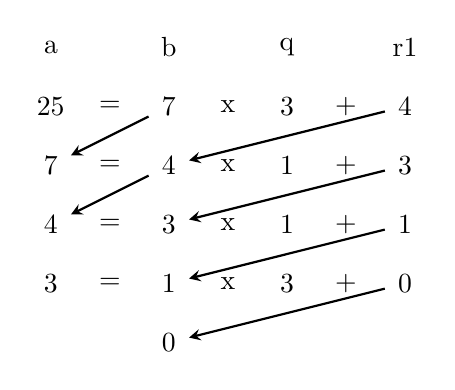
\begin{tikzpicture}[node distance=0.75cm]
  \node (a0) [rsa] {a};
  \node (e0) [rsa, right of=a0] {};
  \node (b0) [rsa, right of=e0] {b};
  \node (m0) [rsa, right of=b0] {};
  \node (q0) [rsa, right of=m0] {q};
  \node (p0) [rsa, right of=q0] {};
  \node (r0) [rsa, right of=p0] {r1};
  
  \node (a1) [rsa, below of=a0] {25};
  \node (e1) [rsa, right of=a1] {=};
  \node (b1) [rsa, right of=e1] {7};
  \node (m1) [rsa, right of=b1] {x};
  \node (q1) [rsa, right of=m1] {3};
  \node (p1) [rsa, right of=q1] {+};
  \node (r1) [rsa, right of=p1] {4};
  
  \node (a2) [rsa, below of=a1] {7};
  \node (e2) [rsa, right of=a2] {=};
  \node (b2) [rsa, right of=e2] {4};
  \node (m2) [rsa, right of=b2] {x};
  \node (q2) [rsa, right of=m2] {1};
  \node (p2) [rsa, right of=q2] {+};
  \node (r2) [rsa, right of=p2] {3};
  
  \node (a3) [rsa, below of=a2] {4};
  \node (e3) [rsa, right of=a3] {=};
  \node (b3) [rsa, right of=e3] {3};
  \node (m3) [rsa, right of=b3] {x};
  \node (q3) [rsa, right of=m3] {1};
  \node (p3) [rsa, right of=q3] {+};
  \node (r3) [rsa, right of=p3] {1};
  
  \node (a4) [rsa, below of=a3] {3};
  \node (e4) [rsa, right of=a4] {=};
  \node (b4) [rsa, right of=e4] {1};
  \node (m4) [rsa, right of=b4] {x};
  \node (q4) [rsa, right of=m4] {3};
  \node (p4) [rsa, right of=q4] {+};
  \node (r4) [rsa, right of=p4] {0};
  
  \node (b5) [rsa, below of=b4] {0};
  
  \draw [arrow] (b1) -- (a2);
  \draw [arrow] (r1) -- (b2);
  \draw [arrow] (b2) -- (a3);
  \draw [arrow] (r2) -- (b3);
  \draw [arrow] (r3) -- (b4);
  \draw [arrow] (r4) -- (b5);
  \end{tikzpicture}
  \end{column}
  \vrule{}
  \column{0.5\textwidth}
  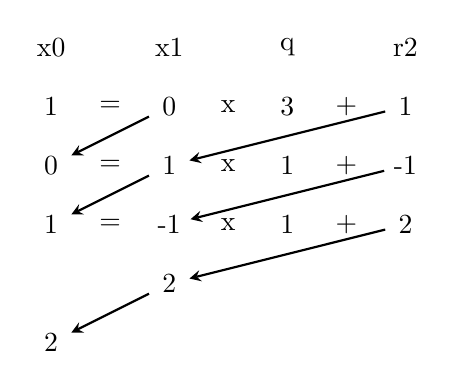
\begin{tikzpicture}[node distance=0.75cm]
  \node (a0) [rsa] {x0};
  \node (e0) [rsa, right of=a0] {};
  \node (b0) [rsa, right of=e0] {x1};
  \node (m0) [rsa, right of=b0] {};
  \node (q0) [rsa, right of=m0] {q};
  \node (p0) [rsa, right of=q0] {};
  \node (r0) [rsa, right of=p0] {r2};
  
  \node (a1) [rsa, below of=a0] {1};
  \node (e1) [rsa, right of=a1] {=};
  \node (b1) [rsa, right of=e1] {0};
  \node (m1) [rsa, right of=b1] {x};
  \node (q1) [rsa, right of=m1] {3};
  \node (p1) [rsa, right of=q1] {+};
  \node (r1) [rsa, right of=p1] {1};
  
  \node (a2) [rsa, below of=a1] {0};
  \node (e2) [rsa, right of=a2] {=};
  \node (b2) [rsa, right of=e2] {1};
  \node (m2) [rsa, right of=b2] {x};
  \node (q2) [rsa, right of=m2] {1};
  \node (p2) [rsa, right of=q2] {+};
  \node (r2) [rsa, right of=p2] {-1};
  
  \node (a3) [rsa, below of=a2] {1};
  \node (e3) [rsa, right of=a3] {=};
  \node (b3) [rsa, right of=e3] {-1};
  \node (m3) [rsa, right of=b3] {x};
  \node (q3) [rsa, right of=m3] {1};
  \node (p3) [rsa, right of=q3] {+};
  \node (r3) [rsa, right of=p3] {2};
  
  \node (a4) [rsa, below of=a3] {};
  \node (e4) [rsa, right of=a4] {};
  \node (b4) [rsa, right of=e4] {2};
  
  \node (a5) [rsa, below of=a4] {2};
  
  \draw [arrow] (b1) -- (a2);
  \draw [arrow] (r1) -- (b2);
  \draw [arrow] (b2) -- (a3);
  \draw [arrow] (r2) -- (b3);
  \draw [arrow] (r3) -- (b4);
  \draw [arrow] (b4) -- (a5);
  \end{tikzpicture}
  \end{columns}
  Với $y0$ tính tương tự. Như vậy, nghịch đảo của $a=25$ trong modulo $b=7$ là 2 ($2*25=50 \equiv 1 \pmod 7$)
\end{frame}

\begin{frame}{Ví dụ RSA I}
\begin{enumerate}
    \item Mã hóa thông điệp $m=15$ với $e=3$, $n=667$
    \item Tìm 2 số $x$, $y$ sao cho $63x+35y=gcd(63, 35)=7 $
    \item Tìm nghịch đảo của 17 modulo 21
    \item Giải mã thông điệp $c=663$, biết $e=3$, $p=23$ và $q=29$
\end{enumerate}
\end{frame}

\begin{frame}{Ví dụ RSA II}
\textbf{Đáp án}
\begin{enumerate}
    \item $c=m^e \pmod n = 15^3 \pmod{667} = 40$
    \item $x=-1, y=2$ thỏa mãn $63*(-1)+35*2=7$
    \item 5
    \item $d=441 \Rightarrow m=c^d \pmod n = 663^{441} \pmod{23*29} = 20$
\end{enumerate}
\end{frame}
\begin{frame}{Hàm băm}
Hàm băm (Hash) $H(x)$ thỏa mãn các yêu cầu sau:
\begin{itemize}
    \item $H$ có thể áp dụng cho các thông điệp $x$ với độ dài bất kì
    \item Kích thước $h=H(x)$ là cố định và nhỏ
    \item Tính một chiều: với một $h$ cho trước, không thể tìm lại $x$ thỏa mãn $h=H(x)$ (về mặt thời gian tính toán)
    \item Tính chống trùng yếu: cho trước một $x$, không thể tìm $y$ thỏa mãn $y \neq x$ và $H(y) = H(x)$
    \item Tính chống trùng mạnh: không thể tìm ra cặp $(x, y)$ bất kì ($x \neq y$) sao cho $H(x)=H(y)$. Nói cách khác nếu $H(x)=H(y)$ thì chắc chắn $x=y$
\end{itemize}

Ví dụ, nếu $x$ chứa 512 bit, còn $h$ là 128 bit thì trung bình sẽ có $2^{512}/2^{128}=2^{384}$ thông điệp $x$ có cùng $h$. Tính chống trùng của hàm Hash là yêu cầu rằng việc tìm ra 2 thông điệp có cùng kết quả Hash là rất khó về mặt thời gian tính toán.
\end{frame}
\begin{frame}{Ứng dụng của hàm băm}
\begin{itemize}
    \item Lưu trữ mật khẩu: trên hệ thống đăng nhập sẽ lưu tên đăng nhập và hash của mật khẩu. Như vậy người quản trị cơ sở dữ liệu sẽ không thể dùng tài khoản của người dùng bất kì để xem trộm thông tin. % Khi người dùng đăng nhập, hệ thống chỉ việc tính hash của mật khẩu nhập vào và so với trên cơ sở dữ liệu
    \item Đấu giá trực tuyến: cơ chế tương tự lưu trữ mật khẩu
    \item Download file: nhiều nhà phát hành phần mềm sẽ để kèm theo hash của file thực thi của phần mềm đó. Chúng ta có thể tính hash của file thực thi đã tải về và so sánh với hash được nhà phát hành công bố. % Nếu không giống tức là file tải về không giống file của nhà phát hành (lỗi đường truyền chẳng hạn)
\end{itemize}
\end{frame}
\begin{frame}{Chữ ký điện tử}
Khi gửi tài liệu (document) đi, chúng ta sẽ thêm vào chữ ký số của file đó (vào phía sau file chẳng hạn)

Khi người nhận được tài liệu sẽ tiến hành kiểm tra bằng việc kiểm tra chữ ký đó, từ đó biết được tài liệu có bị lỗi không

\begin{tikzpicture}[node distance=1.25cm]
\node (doc) [data] {Tài liệu (Document};
\node (sign) [function, right of=doc, xshift=1.5cm] {Ký (Sign)};
\node (true) [data, right of=sign, xshift=1.5cm] {Đúng};
\node (signature) [data, below of=sign, yshift=-1cm] {Chữ ký};
\node (verify) [function, right of=signature, xshift=1.5cm] {Kiểm tra (Verify)};
\node (false) [data, right of=verify, xshift=1.5cm] {Sai};
\draw [arrow] (doc) -- (sign);
\draw [arrow] (sign) -- (signature);
\draw [arrow] (signature) -- (verify);
\draw [arrow] (verify) -- (true);
\draw [arrow] (verify) -- (false);
\end{tikzpicture}
\end{frame}
\begin{frame}{Phương pháp trao đổi khóa}
Ý tưởng chung của các phương pháp trao đổi khóa như sau:
\begin{columns}
\column{0.4\textwidth}
\begin{figure}
    \includegraphics[scale=0.1]{diffie-hellman.png}
    \caption{Wikipedia}
\end{figure}

\column{0.6\textwidth}
\begin{enumerate}
    \item Alice và Bob thống nhất 1 khóa chung \textbf{G} (màu vàng)
    \item Alice chọn khóa bí mật \textbf{A} (màu đỏ) và Bob chọn khóa bí mật \textbf{B} (màu xanh)
    \item Alice tính khóa công khai của mình là \textbf{G+A} và gửi cho Bob. Bob tính khóa công khai của mình là \textbf{G+B} và gửi cho Alice
    \item Từ khóa công khai \textbf{G+B} của Bob, Alice tính được \textbf{G+B+A}
    \item Từ khóa công khai \textbf{G+A} của Alice, Bob tính được \textbf{G+A+B}
    \item Bây giờ Alice và Bob đều có \textbf{G+A+B} và sử dụng nó là khóa cho mã hóa đối xứng.
\end{enumerate}
\end{columns}
\end{frame}
\begin{frame}{Kiến thức nền tảng}
\begin{enumerate}
    \item Khoa học máy tính
    \begin{itemize}
        \item Lập trình (C/C++/Python)
        \item Cấu trúc dữ liệu và giải thuật (bruteforce)
        \item Mạng máy tính (giao thức bảo mật web, mạng)
    \end{itemize}
    \item Toán
    \begin{itemize}
        \item Đại số tuyến tính (Linear Algebra)
        \item Lý thuyết số (Number Theory)
        \item Toán trừu tượng (Abstract Algebra)
    \end{itemize}
\end{enumerate}
\end{frame}
\begin{frame}{Khoa học máy tính}
\begin{enumerate}
    \item Lập trình: khuyến khích sử dụng các ngôn ngữ scripting, code ngắn gọn, nhiều thư viện hỗ trợ, như Python, Ruby, Rust, ...
    \item Biểu diễn dữ liệu trên máy tính: hệ cơ số 10, 2, 8, 16
    \item Encode và Decode: base64, base32, ....
    \item Cấu trúc dữ liệu và giải thuật
    \begin{itemize}
        \item Bruteforce
        \item Chia nhị phân
        \item Danh sách, Cây nhị phân
    \end{itemize} 
    \item Mạng máy tính
    \begin{itemize}
        \item Lập trình socket (với Python)
        \item Giao thức HTTPS
    \end{itemize}
\end{enumerate}
\end{frame}
\begin{frame}{Toán I}
\begin{enumerate}
\item Đại số tuyến tính
\begin{itemize}
    \item Ma trận. Các phép toán trên ma trận. Định thức
    \item Không gian vector. Cơ sở. Chiều
    \item Ma trận trực giao. Ma trận trực chuẩn
    \item Chéo hóa ma trận
    \item ....
\end{itemize}
\item Lý thuyết số
\begin{itemize}
    \item Đồng dư thức modulo. Thuật toán tính $a^n \pmod p$ nhanh
    \item Ước chung. Bội chung. Thuật toán Euclid. Thuật toán Euclid mở rộng và nghịch đảo trong modulo $p$
    \item Phi hàm Euler. Định lý Euler. Định lý Fermat
    \item Định lý số dư Trung Hoa (Chinese Remainder Theorem)
    \item Số chính phương modulo $p$ nguyên tố (Quadratic Residue)
\end{itemize}
\end{enumerate}
\end{frame}
\begin{frame}{Toán II}
\begin{enumerate}
\item Toán trừu tượng
\begin{itemize}
    \item Lý thuyết nhóm. Định nghĩa. Tính chất của nhóm, vành, trường. Ví dụ và giải thích
\end{itemize}
\item Toán rời rạc
\begin{itemize}
    \item Đại số Boolean
\end{itemize}
\item Xác suất thống kê
\end{enumerate}
\end{frame}

\begin{frame}{Kỹ năng cần có}
    \begin{enumerate}
        \item Lập trình
        \item Đọc hiểu code
        \item Research về code, về toán, ....
    \end{enumerate}
\end{frame}
\begin{frame}{Examples}
\begin{enumerate}
    \item Viết chương trình tính ước chung lớn nhất của 2 số sau: 420 và 852
    \item Đoạn code sau làm gì?
    \lstinputlisting[firstline=1, lastline=12, language=Python]{hill.py}
\end{enumerate}
\end{frame}

\begin{frame}{Đáp án Examples}
\begin{enumerate}
    \item $gcd(420, 852) = gcd(852, 420) = gcd(420, 12) = gcd(12, 0) = 12$
    \item Mỗi ký tự in thường được trừ đi 97 (mã ascii của "a") để nằm trong khoảng 0 ... 25. Mỗi vòng lặp đoạn code mã hóa 2 kí tự cùng 1 lúc như sau:
    \begin{itemize}
        \item \textbf{key} là 1 ma trận 2x2 $\begin{bmatrix}k_{00} & k_{01} \\ k_{10} & k_{11}\end{bmatrix}$
        \item Ciphertext ở vị trí \textbf{i} và \textbf{i+1} được mã hóa bằng plaintext ở 2 vị trí đó bằng công thức: $\begin{bmatrix}c_i \\ c_{i+1}\end{bmatrix} = \begin{bmatrix}k_{00} & k_{01} \\ k_{10} & k_{11}\end{bmatrix} \begin{bmatrix}p_i \\ p_{i+1}\end{bmatrix}$
        \item Cuối cùng cộng lại cho 97 để trở thành ký tự in thường
    \end{itemize}
\end{enumerate}
\end{frame}
\end{document}